\section{Problem Definition and Related Work}
%\section{Network Uncertainty}
\label{sec:motivation}

%We want to ensure that networks are always in correct states over time and state changes.

%Our ultimate goal is to ensure that networks are always in the correct states over time and state changes, specifically in the context of SDN, in which a logically centralized controller is responsible for disseminating commands to network devices with the following three objectives.
%There are three key goals of our work, which we discuss in the following subsections:

%\kevin{To ensure that networks are always in the correct states over time and network state changes, we design \name to achieve the following three objectives.}

\matt{We design \name to achieve the following \cut{three }objectives:}

\if 0
\begin{itemize}
%\item Consistency during network updates at every step (\S\ref{sec:everystep}),
\item Consistency during network updates (\S\ref{sec:everystep}),
\item With efficient update installation (\S\ref{sec:efficient}), and
\item Customizable network consistency properties (\S\ref{sec:general}).
%\item to handle general network consistency properties;
%\item to enforce consistency during network updates;
%\item to maximize update efficiency.
\end{itemize}
\fi

%\subsection{Consistency at Every Step}
%\label{sec:everystep}
\paragraphb{1) Consistency at Every Step.}
\wxzcr{Network changes can occur frequently, \cut{expecially in SDNs, }triggered by the control applications,
changes in traffic load, system upgrades, or even failures.}
\wxzcrnew{Even in SDNs with a logically centralized controller,}
the asynchronous and distributed nature\cut{ of modern networks} implies that no single
component can always obtain a fully up-to-date view of the entire system.
%always obtain a correct instantaneous network-wide view. 
%The emergence of SDN, despite providing a logically centralized management interface, 
%does not change that fact~\cite{Nice2012}. \fixme{What fact are we backing up with that citation?}
%Thus, our observation of a network, for example, from an SDN controller, is uncertain at any given time. 
%The root cause is the inevitable delays between the controller and network devices,
%, as well as the unpredictable  \wxzc{as well as rule installation time}
%which vary across devices and over time.
%After issuing updates to the network, the controller has 
%limited knowledge about the exact timing and ordering with which the updates will be applied. 
%After network changes occur, such as device failures, link congestion, and end-hosts migrations, the controller will be aware of those changes only after a certain
%delay, or may never learn of them, depending on the implementation.  
Moreover, data packets from all possible sources may traverse the network at any time in any
order, interleaving with the network data plane updates. 
How can we continuously enforce consistency properties, given the incomplete and uncertain network view at the
controller? 
%\wxz{One group of approaches, taken in prior work~\cite{Reitblatt2012, incremental-cu, zUpdate,
%Hong13, OFCPP}, carefully transitions network states such that intermediate
%states remain consistent.} However, those solutions do not handle generalized properties, %\cut{and result in slow updates}
%\wxznew{and/or slow the network update process}.

%nor produce good update efficiency.  \wxz{For example, CU (CU)~\cite{Reitblatt2012} makes sure no packet sees a mix of old and new network states during transitions via a two-phase update scheme. Its update process is paused after the first phase until making sure all the issued updates are applied.  What's more, packets handled by each configuration are tagged with different version numbers to avoid encountering a mix of configurations.  CU does not delete old rules until making sure that all in-flight packets processed by the old configuration drain out of the network. 

%In practice, it takes time for controller to issue each command, 
%and  network-wide update in large-scale networks  
%they don't handle general consistency policies efficiently.
%\wxz{In particular, CU~\cite{Reitblatt2012} 

%In this way, CU guarantees that packet behaviors satisfy a property at every step during network configuration changes, as long as the start and final state satisfy the property. But this comes at the price of efficiency and with a rigid notion of consistency as we will see in the following sections.}

%\subsection{Customizable Consistency Properties}
%\label{sec:general}
\paragraphb{2) Customizable Consistency Properties.}
Moreover, the range of desired consistency properties of networks is quite broad and diverse. 
For example,
the successful operations of some networks 
may depend on a set
of paths traversing a firewall, certain ``classified" hosts being
unreachable from external domains, enforcement of access control to
ensure critical assets, balanced load across links, loop freedom, etc..
%depend on loop freedom, balanced
%load across links, use of optimal routes, enforcement of access control to
%secure critical assets, or a combination of several of these.
%Existing mechanisms deals with different consistency properties, individually.
%and their focuses are in isolation.
As argued in~\cite{Mahajan13}, a generic framework to handle general properties
is needed.  Researchers have attempted to ensure certain types of consistency
properties, e.g., loop freedom, absence of packet
loss~\cite{zUpdate, zUpdate, Hong13}, 
but those studies do not provide a generalized solution.
\wxznew{Dionysus~\cite{jin2014dynamic}, as stated earlier, generalizes the scope of 
consistency properties it deals with, but still requires designing 
specific algorithms for different invariants.}
\wxzcrnew{Consistent Updates~\cite{Reitblatt2012} is probably the closest solution to
support general consistency properties, but as we will see next, it sacrifices efficiency.}
%\subsection{Efficient Update Installation} 
%\subsection{Maximizing Control Throughput} 
%\label{sec:efficient}

\paragraphb{3) Efficient Update Installation.}
%Network changes in SDN can occur frequently, triggered by the control applications,
%changes in traffic load, system upgrades, or even failures.
%Accordingly, they 
\pbg{The network controller should} react in a timely fashion to network changes 
to minimize the duration of performance drops and network errors.
% (e.g., low network utilization, congestion, or data loss). 
%As indicated in \cite{jin2014dynamic}, many systems (see \cite{jain2013b4, Hong13} for wide-area solutions, and
%\cite{al2010hedera,benson2011microte,curtis2011devoflow} for data center solutions) dynamically change the network based on workload, and the system efficiency is
%highly dependent on how fast the network can be updated.
%In modern networks with high data rate links, even a few milliseconds delay of applying updates can cause thousands of connections to back off or undergo major outages.\wxzc{A reviewer doubted this fact.}
%Consider the scenario where a terabit link is congested and this causes the controller to issue updates to migrate some flows from that link. A few milliseconds delay of applying the updates may affect 1000+ of connections to majorly backoff.  }
%That is, }correctness and efficiency are two sides of the same coin, 
%and both are crucial to network management. 
There have been proposals~\cite{Reitblatt2012, incremental-cu, zUpdate, Hong13, noyes2014toward} that instill correctness according to a specific consistency property, but these approaches suffer substantial performance penalties. 
For example, 
\wxzcrnew{the waiting time between phases using the}
two-phase update scheme proposed in CU~\cite{Reitblatt2012} is at least the maximum delay across all the devices, assuming a completely
parallel implementation. \pbgc{Rephrase}
%\cut{While preserving correctness properties, network
%operators also wish to perform network operations in the most efficient manner.}
Dionysus \cite{jin2014dynamic} was recently proposed to update networks via dynamic scheduling atop a consistency-preserving dependency graph.
%\cut{ 
%For each particular invariant, Dionysus requires a dependency graph and an algorithm specific to that invariant. For example, a packet coherence invariant needs one algorithm and a waypoint invariant would need a new algorithm.}
However, it requires implementing a new algorithm and dependency graph for each new invariant to achieve good performance. 
For example, a packet coherence invariant needs one algorithm and a waypoint invariant would need another algorithm.
%'s efficiency 
%depends on how specific the algorithm that generates the graph is to the invariant one cares about. 
%For example, if an operator only wants to enforce a waypointing invariant, but uses the default algorithm to generate a graph that ensures packet coherence. Then network update efficiency wound not be maximized.
In contrast, our approach reduces the consistency problem to a general network verification 
problem, which can take a broad range of invariants as inputs.
In particular, one only needs to specify the verification function instead of designing 
a new algorithm. % to automatically generate the dependency graph.
 %Our approach is to convert the complex scheduling problems to general network verification problems, in which operators only need to specify the verification function instead of designing a new algorithm to automatically generate the dependency graph. 
This approach also grants \name the ability to deal with wildcard rules efficiently, 
in the same way as general verification tools, 
whereas Dionysus only works for applications with
%non-wildcard rules.
exact match on flows or classes of flows.
%\wxzcr{A more recent approach~\cite{mcclurg15} reduces update overhead via allowing customized policies, which are restricted to trace-based properties weaker than packet coherence.} \pbgc{You could move that discussion of~\cite{mcclurg15} to the related work.}
%For example, it is straightforward to handle overlapped rules (with longest prefix match) in \name than in Dionysus, since verifying the properties is easy.
 %\if 0
 %Take CU~\cite{Reitblatt2012} again and incremental CU (Incremental-CU)~\cite{incremental-cu} as
 %examples.  \wxz{ As discussed previously, using CU,
 %%makes sure no packet sees a mix of old and new network states during transitions (packet coherence) via a two-phase update scheme.
 %network update process is divided into two phases, and paused after the first
 %phase until making sure all the issued updates have been processed.  For each
 %update, the controller is only able to confirm it after a round trip time
 %between the controller and the device where the update is applied, plus the
 %processing time at that device.  Thus, the total waiting time between the two
 %phases is the maximum delay across all the devices, assuming a completely
 %parallel implementation. 
 %%In practice, it takes time for controller to issue each command, 
 %%and  network-wide update in large-scale networks  
 %%they don't handle general consistency policies efficiently.
 %%What's more, packets handled by each configuration are tagged with different version numbers to
 %%avoid encountering a mix of configurations.
 %CU maintains old configuration rules until all in-flight packets processed by
 %the old configuration leave the network.  } As a result, CU demands to double
 %the storage space for each updated rule in network device memory, e.g., TCAM
 %memory, which is expensive and power-consuming. To address this, incremental
 %consistent updates (Incremental CU)~\cite{incremental-cu} is proposed to trade
 %time with flow table spaces. By breaking a batch of updates into $k$ subgroups,
 %incremental-CU manages to reduce the extra memory usage to roughly $1/k$, but
 %takes much longer time to apply all the updates ($k$ times the delay using CU).
 %\fi
%Let us consider a control application which reactively assigns paths in response to data flow arrivals.
%As a stream of flows arrive, the operator %cannot afford waiting 
%needs to wait for the two-phase update delay (taking at least one and half round trip times between the controller and switches plus the rule installation time) before allowing each flow to enter the network.

 %\if 0
 %However, aforementioned schemes, like CU, preserve a fairly rigid requirement,
 %which may not always be suitable for applications.  On one hand, the
 %application might need less than CU provides, i.e., CU is enforcing a much
 %stronger policy than is necessary.  It is quite possible that the system only
 %needs a much lower level of consistency, e.g., absence of loops, to be
 %maintained during transitions.  In that case, as long as no loops are formed,
 %it doesn't matter that flows are processed by a mix of old and new
 %configurations, so we don't need to delay most updates.  As discussed in
 %~\cite{Mahajan13}, 
 %%the timing of safely applying 
 %%one update is dependent on existing updates in the data plane.
 %the higher level the enforced consistency property is,
 %%(e.g., packet coherence is a stricter requirement than loop freedom), 
 %the stronger dependency is imposed among the rules, 
 %and thus, the slower the data plane can be updated.
 %%Hence, it opens the opportunity to perform more efficient updates with a solution tailored to the actual need of the application.
 %On the other hand, the application might need more than what CU can provide,
 %for example, no more than a certain number of flows congesting a bottleneck
 %link.  Hence, there is an opportunity to perform more efficient updates with a
 %solution tailored to the actual need of the application.
 %
 %%- Mention there is general-purpose verification, but�
 %%* Does not take into account temporal uncertainty
 %%* Verification does not preserve a property, just checks for it
 %\fi
%\kevin{Finally, there are also tools~\cite{Al-Shaer2010, NetPlumber2013, VeriFlow} that attempt
%to check network state snapshots incrementally for {\em general} properties, and
%optionally block faulty updates, 
%but they do not provide a mechanism to instill more general notions of consistency or correctness.
%%but they do not instill correctness. 
%%The difference between our work and these earlier works is that we focus on achieving the {\em generality} of the consistent properties that a system needs to maintain as well as the high {\em efficiency} (fast update speed and
%%small memory requirement) needed to process network updates.}
%}

%It no longer pre-determines a schedule, but still requires planning the dependency graph ahead. 
%\kevinc{I am a bit confusing about the previous sentence , (1) we already say it is dynamic scheduling, (2) we may want to say planning of what ahead, the dependency graph?} 

%but such network models without considering the temporal uncertainty will lead
%to inaccurate network behavior. 
%Moreover, other than verification and blocking, they do not try to instill correctness.

%No matter what properties a system cares about, 
%the same heavy update mechanism is applied.

%In those cases, using such schemes will result in unnecessary costs in terms of both latency and device memory consumption.
%Therefore, subject to consistency property constraints,
%maximizing control throughput to speed up processing of updates is of great importance. 

%Moreover, various functionalities of modern networks could require arbitrary properties, 
%and as a network evolves, its required properties may change. 
%Together these requirements demand a light-weighted network updating method 
%that supports a generic set of consistency properties. 
%One approach would be to implement a general consistency enforcement mechanism from scratch. 
%However, there has been extensive work on general network verification~\cite{HSA, VeriFlow, NetPlumber2013, Al-Shaer2010, Anteater}. Hence, we took the approach of developing a scheme to %``reduce and 
%translate consistency enforcement into network verification (\S~\ref{sec:design}).

%First, some networks may need diffrent
%properties, for which effective procedures or even best-
%case structures are unknown (e.g., load balancing across
%links and maintaining packet ordering within a flow)

%Second, even for the properties in Table
%focuses on consistency properties in isolation. 
%The combinations are hard to ensure, and everycient algorithms are not
%known. For instance, drop freedom and memory limit,
%while easy to ensure individually, are challenging to en-
%sure in combination. Maintaining the combination re-
%quires global dependencies, as introducing some rule
%at a switch might need to remove another rule first,
%which can only be removed after having added a new
%rule somewhere else
%Third, the table only shows the qualitative part of
%the story and ignores quantitative ects that may be
%equally important. Even though [
%] can resolve the dependencies

%In this section, we describe the problem of network uncertainty and its negative effect on network-wide verification. 
%Here, we define the inconsistency between the view of the observation point and the network state data packets encounter as network uncertainty.

%Such uncertainty imposes an question to network verification, and more specifically, here we focus on data plane verification by analyzing snapshots of the network-wide data-plane state~\cite{Al-Shaer2009, Al-Shaer2010, VeriFlow, PHA2012, NetPlumber2013}. \emph{What if there is uncertainty of the presentation of the network snapshots?} Before answering this question, we first illustrate how badly this uncertainty can affect network verification.
%
%First, the bugs caused by such uncertainty, and thus neglected by the current data-plane verifiers, are prevalent. 
%%To illustrate how uncertainty makes the problem much harder,
%
%\begin{figure}[!ht]
%  \centering
%  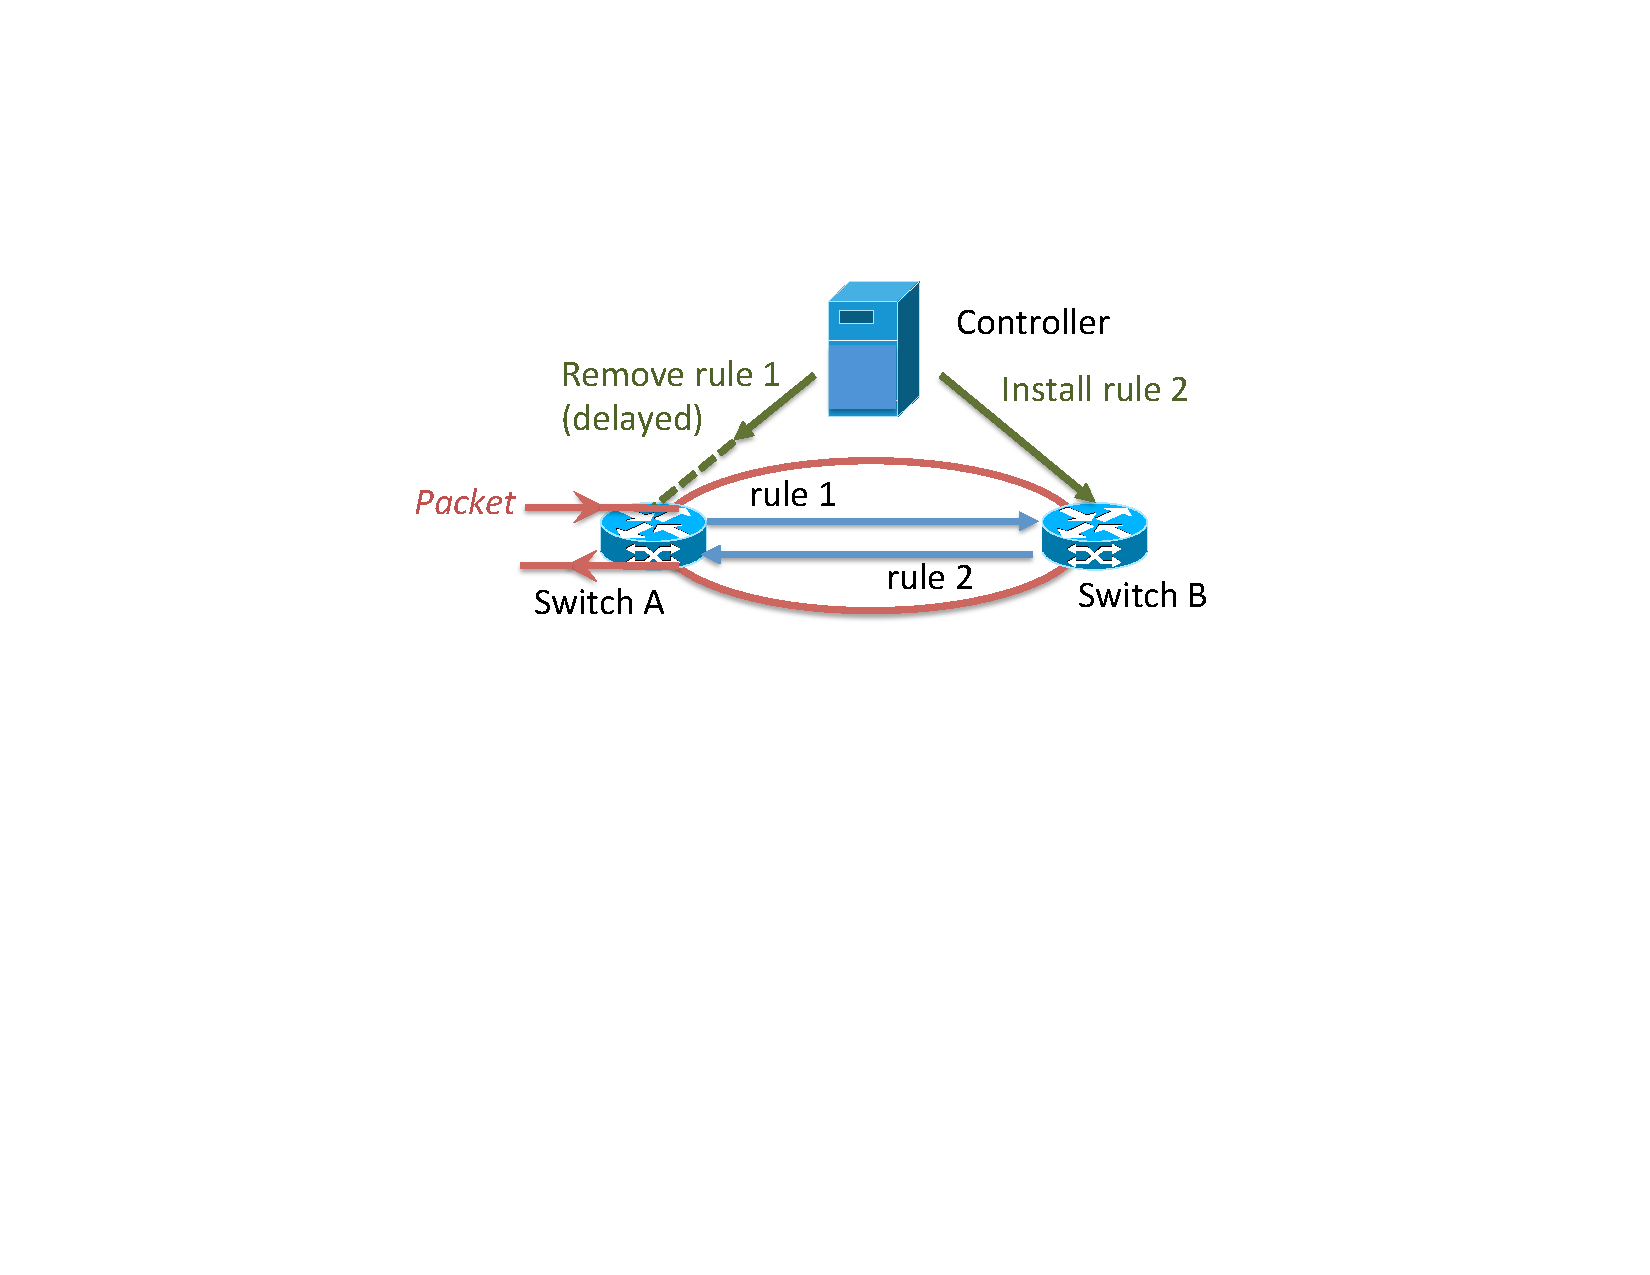
\includegraphics[width=\columnwidth]{figs/example}
%  \caption{Example.}
%  \label{fig:example}
%\end{figure}
%
%Let us look at an extremely simple example (Figure~\ref{fig:example}). Suppose there are two switches, $A$ and $B$, in the network, and switch $A$ has a forwarding rule to $B$. For the sake of simplicity, assume $A$ forwards all packets to $B$. Now the network operator wants to reverse the flow of traffic through the following two steps: 1. telling switch $A$ to remove its flow rule; 2. telling switch $B$ to insert a flow rule sending everything to $A$. Now the operator issues these two commands in this order, and neither the before or the after state of the network contains a loop between $A$ and $B$. However, we do not know when the commands arrive and are processed. It is possible that the execution on switch $B$ happens earlier than that on switch $A$, resulting a transient loop. This bug may seem not quite harmful, but the consequence of ignoring it could induce a chain of errors, especially when this transient state lasts long enough. Besides, this shows even such a simple task which is well planned in advance can go wrong due to some uncertainty. 
%%Note that in this case, serializing rule installation would help eliminate the bug, but at the cost of performance, and more importantly there are scenarios where carefully crafting ordering doesn't help~\cite{Reitblatt2012}. More devastating examples include errors caused by interleaving between packet arrivals and configuration changes, which will be discussed in more details in Section\ref{sec:motivation}.
%As for commonly used control programs, things are the same. 
%Three out of eleven bugs found by NICE~\cite{Nice2012}, (BUG-V, BUG-IX, and BUG-XI) are caused by the control programs' lack of knowledge of the network sate.  
%
%Second, such bugs may bring serious consequences.
%One may think such uncertainty related errors are all transient, and as a result, ignoring them doesn't matter much. 
%This is true with this reversing link example. 
%However, some such errors can be permanent if no attention is paid. 
%For example, if the control program asks a switch to install a rule at some point, 
%but later the program wants to withdraw this rule. 
%The problem is the two instructions can be reordered at the switch, 
%and what the switch does is first to remove a non-existing rule, 
%and then install the same rule, resulting a state against the program's intention. 
%Without querying the flow table at the switch, 
%the view of the controller and the network state will be inconsistent until the rule expires.
%One may argue that inserting a barrier message in between the two instructions solves the problem. 
%But first, this is only an example to demonstrate the point for the sake of simplicity, 
%and realistic cases are much more complex. 
%While in this case, serializing rule installation would help eliminate the bug at the cost of performance, 
%there are scenarios where carefully crafting ordering doesn't help~\cite{Reitblatt2012}. 
%Besides, it is the question who should be responsible to discover this problem and to insert the barrier message.
%As for commonly used control programs, things are the same. 
%Three out of eleven bugs found by NICE~\cite{Nice2012}, (BUG-V, BUG-IX, and BUG-XI) are caused by the control programs' lack of knowledge of the network sate.  
%
%Moreover, even if the errors disappear after a while, they have the potential to make the network suffer in terms of both security and performance. 
%%performance
%%security
%As for security, temporary access control violation may result that malicious or untrustworthy packets enter a secure zone~\cite{Reitblatt2012}. 
%%Another example is stateful firewall....
%For performance, take the previous example again. 
%If a packet enters switch $A$ while the forwarding loop exists. Note that in a realistic deployment, switches will refuse to forward packets back through their ingress port, but drop them. So the packet encounters a black hole at switch $B$ instead of a loop. A recent study~\cite{Flach2013} shows that TCP transfers with loss may take five times longer to complete compared with connections with no loss. That is, such bug may cause significant performance drop.
%%\cite{OFCPP}
%
%We conduct some measurement study to show how seriously network uncertainty can cause performance drop. Results are shown in \S~\ref{sec:bug-coverage}. 
%

%\subsection{Related Work}
%\paragraphb{Related Work.}
\if 0
\wxznew{
To rigorously check network correctness,
\cut{ software or configurations.} 
researchers have investigated various network verification techniques, such as symbolic execution~\cite{holzmann2004primer} and configuration file analysis~\cite{visser2003model, vasic2011identifying}.
\cut{
Symbolic execution
\cite{holzmann2004primer} is used to catch bugs through exploration of all possible
code paths, but is usually not tractable for large software.  Analysis of
configuration files ~\cite{visser2003model, vasic2011identifying} also helps,
but fails to find bugs in software of networking devices, and is designed
for specific configuration languages and control protocols. }
Another approach is to statically analyze snapshots of the network state 
in an off-line \cite{wang2011openflow,
heller2010elastictree, mk+sigcomm+11, cadar2008klee, baier2008principles,
flanagan2005dynamic, PHA2012} or an on-line manner
\cite{NetPlumber2013, Al-Shaer2010, VeriFlow, yang2013real}.
%. However, those previous approaches operate
%offline, and thus, find bugs only after they happen. Online verification tools
%are also developed \cite{NetPlumber2013, Al-Shaer2010, VeriFlow} to check
%dynamic snapshots in real time. 
%However, none of the existing tools take
%uncertainty caused by network dynamics into consideration.
This approach is scalable, protocol agnostic and able to catch bugs in network device software, but none of those methods consider temporal uncertainty during the transition of the snapshots. Instead, they effectively but incorrectly assume that the updates are applied at the exact moment when the verification tools see them.  
}
\fi

\if 0
Another train of inquiry \cite{incremental-cu,Reitblatt2012, zUpdate, Hong13}
focuses on how to synthesize a correct update plan to avoid inconsistencies, which may cause transient faults in the network.
Nonetheless, these solutions could be expensive in time and flow table usage and/or update delay, and they}
%However, their solutions are too expensive to achieve real-time performance
%with heavy flow table storage usage or long updates buffering time. 
%In addition, the existing approaches 
are not designed to be flexible enough to enforce generic network invariants. 
Reitblatt et al. \cite{reitblatt2013fattire} also proposed a language based on regular expressions for synthesizing
fault-tolerant network programs, but the operations have to be performed
offline.
\fi

\if 0
\kevin{Another train of inquiry focuses on how to synthesize a correct update
plan to avoid inconsistencies\cut{, which may cause transient faults in the network}.
Reitblatt et al.~\cite{Reitblatt2012} propose a two-phase update scheme to
preserve packet coherence\cut{and reachability-based invariants in SDN}.
Katta et al. \cite{incremental-cu} manage to reduce the memory requirements of
CU at the cost of longer delay. Peresini et al.~\cite{OFCPP}
propose a multi-commit transactional semantic at the controller for ensuring
consistent packet processing. Noyes et al. offer a tool to generate updates
for maintaining user-specified invariants \cite{noyes2014toward}. Researchers have
also investigated ways to preserve bandwidth-based invariants during network
transitions~\cite{zUpdate, Hong13}. The difference between our work and that earlier work is that we focus on the {\em generality} of the consistency properties that a
system needs to maintain as well as the high {\em efficiency} (fast update speed and
small memory requirement) needed to process network updates.}

Dionysus \cite{jin2014dynamic} is recently proposed to address the
efficiency issue of updating networks under general consistency requirements,
via dynamic scheduling on top of a consistency-preserving dependency graph,
which requires to be planned ahead.
%It no longer pre-determines a schedule, but still requires planning the dependency graph ahead. 
%\kevinc{I am a bit confusing about the previous sentence , (1) we already say it is dynamic scheduling, (2) we may want to say planning of what ahead, the dependency graph?} 
We take a different approach by converting complex scheduling problems to well-defined network verification problems.
\fi

%efficiency of general CU based on dynamic scheduling atop a
%consistency-preserving dependency graph. We take a different approach by
%converting the complex scheduling task into a generic verification problem.
\cut{ As discussed in ~\cite{Mahajan13}, the higher level the enforced
consistency property is, the stronger dependency is imposed among the rules,
and thus, the slower the data plane can be updated. Our black-box approach is
not only general, but also offers operators the flexibility to balance the
speed and consistency level, instead of pausing the system for strict but
unnecessary consistency enforcement. } 

\if 0
Other researchers have also noticed the problem of inconsistent view between
SDN-controller and the network states. Peresini et al.~\cite{OFCPP} proposes a
multi-commit transactional semantic at the controller for ensuring consistent
packet processing. Heller et al.~\cite{sdnlayering} presents a big picture of
cross-layer diagnostic framework for systematic troubleshooting in SDNs, and
rigorous network-wide verification which we have explored in this paper, is an
essential component towards that goal. 
\fi
%4. Stateful firewall (logic programming for SDN)	
%
%The key idea: the domain is able to send any traffic to the outside world, while an outside entity is only allowed to send traffic into the domain if the domain has first sent it a packet. 
%
%Model: one switch with two ports. Port 1: the external world, port 2 internal.
%Any pkt that arrives on port 2 is routed to port 1. In addition, the firewall remembers the dst IP of such a packet. 
%Any packet that arrives on port 1 is dropped unless the src IP matches one of the IPs that it has remembered. In this latter case, it forwards the pkt to port2.
%
%
%Default rule: any traffic that comes in on port 2 to be forwarded out on port 1
%Each pkt with a unique dst IP arriving at port 2 should be sent to the controller. When such a packet is processed, the run-time system extracts the dst IP and stores it as seen, and generates a specific rule that all traffic appearing on port 1 whose srcip field is IP is forwarded out port 2.
%
%Events: 1. client sends a pkt to server
%
%	2. SW sends this pkt to Controller
%
%3. Controller sees the pkt, stores dst ip IP, installs a rule that allows pkt whose srcip == IP from port1 to port2
%
%In VF: 	Init: 	for EC (c-->s) c-->SW-->s
%
%for EC (s-->c) c     SW<--s 
%
%after event 3, for EC (c-->s) c-->SW-->s
%
%for EC (s-->c) c<--SW<--s 
%
%But in reality, rule could arrive at SW after server’s response
%
%then for this pkt, EC(s->c) still c  SW<--s
%
%could be detected by VF with uncertainty

